\documentclass[10pt,twocolumn]{article}

\usepackage[letterpaper,margin=0.75in]{geometry}
\usepackage{times}
\usepackage{url}
\usepackage{xurl}
\usepackage{hyperref}
\usepackage{booktabs}
\usepackage{amsmath}
\usepackage{amssymb}
\usepackage{graphicx}
\usepackage{caption}
\usepackage{subcaption}
\usepackage{multirow}
\usepackage{xspace}
\usepackage{enumitem}

\newcommand{\SystemName}{\textsc{QSupremacy}\xspace}
\newcommand{\cuQuantum}{\texttt{cuQuantum}\xspace}
\newcommand{\Perlmutter}{\texttt{Perlmutter}\xspace}
\newcommand{\todo}[1]{\textbf{TODO: #1}}

\title{\SystemName: Modeling Application-Level Quantum Advantage over Native HPC}

\author{Anonymous Authors}
\date{}

\begin{document}
\maketitle

\begin{abstract}
Quantum advantage is often discussed through asymptotic algorithmic speedups or through the cost of simulating quantum circuits on classical machines. For HPC users, however, the practical question is application-level: when does a quantum-circuit version of an application outperform the best native HPC implementation of the same task?

This paper presents \SystemName, a Perlmutter-based methodology for modeling application-level quantum advantage. \SystemName compares native ML/HPC application paths against quantum-circuit application paths executed with \cuQuantum, then projects the quantum hardware requirements needed to beat the native path. Following our prior accepted systems papers, the paper is organized around a clear gap: native HPC baselines are strong, quantum-circuit applications incur nontrivial encoding and execution overheads, and the break-even hardware region must be measured rather than assumed. Our first workload suite targets \texttt{sklearn digits}, quantum kernel classification, and QNN/VQC classification under a shared time-to-quality policy. Results are pending; this draft defines the logical structure, system design, and evaluation plan.
\end{abstract}

\section{Introduction}

Quantum computing offers a computational model distinct from classical computing by operating on qubits rather than binary bits. Superposition and entanglement enable circuit structures that can express computations differently from native CPU/GPU programs. These properties motivate quantum algorithms for simulation, optimization, cryptography, and machine learning. Despite this promise, current devices remain constrained by noise, limited qubit counts, short coherence times, and expensive access. As a result, practical quantum advantage for real applications remains an open systems question rather than a settled hardware fact.

High-performance computing systems have therefore become the practical platform for studying quantum applications before fault-tolerant quantum hardware is available. Libraries such as \cuQuantum allow researchers to execute quantum circuits on GPU clusters, measure circuit-level costs, and prototype hybrid quantum-classical applications. However, using HPC to simulate a quantum circuit does not by itself establish quantum advantage. A simulator can be faster than another simulator while the quantum-circuit application remains slower than a native classical implementation of the same task.

\begin{figure}[t]
    \centering
    \fbox{\parbox{0.92\linewidth}{\centering
    Placeholder: end-to-end comparison of native ML, quantum kernel, and QNN/VQC paths on the same workload.}}
    \caption{Application-level comparison target. The central comparison is not NumPy state-vector simulation versus \cuQuantum, but native application execution versus quantum-circuit application execution and projected hardware execution.}
    \label{fig:intro-gap}
\end{figure}

Figure~\ref{fig:intro-gap} summarizes the gap that motivates this work. Native HPC/ML frameworks execute directly on GPUs and benefit from decades of optimization. Quantum-circuit applications require feature encoding, circuit construction, repeated circuit execution, measurement or observable extraction, and classical postprocessing. These stages can dominate the total time, especially for machine-learning workloads where many samples, shots, and optimizer iterations are required. Thus, quantum advantage should be evaluated as an end-to-end application question: for the same dataset, target quality, and system budget, when does the quantum-circuit path win?

Prior work from our group has studied large-scale quantum simulation systems. ScaleQsim improves distributed full state-vector simulation on leadership-scale GPU systems~\cite{scaleqsimtodo}, while AURORA-Q extends simulation capacity through tiered-memory and asynchronous offloading~\cite{auroraqtodo}. These systems answer how to make quantum circuit simulation scale on HPC resources. \SystemName asks the next question: given these simulation capabilities, what do they imply about application-level quantum advantage over native HPC?

\begin{table}[t]
\caption{Positioning of \SystemName relative to prior work.}
\centering
\small
\resizebox{\columnwidth}{!}{%
\begin{tabular}{lccc}
\toprule
System & Simulation scale & Resource model & App-level advantage \\
\midrule
ScaleQsim & \checkmark & GPU/node scaling & -- \\
AURORA-Q & \checkmark & Tiered memory & -- \\
cuQuantum & \checkmark & GPU kernels & -- \\
\SystemName & \checkmark & Allocation-aware & \checkmark \\
\bottomrule
\end{tabular}
}
\label{tab:intro-position}
\end{table}

Table~\ref{tab:intro-position} shows the intended positioning. \SystemName does not replace simulator optimization work. Instead, it uses simulator measurements as one layer in an application-level model that includes native baselines, quantum encoding overheads, repeated circuit execution, Slurm allocation costs, and projected quantum hardware parameters.

In this paper, we present \SystemName, an application-level quantum advantage modeling framework for HPC systems. \SystemName uses a shared workload definition to execute three paths: native ML baselines, quantum kernel classifiers, and QNN/VQC classifiers. It measures runtime, quality, circuit metadata, and allocation cost on \Perlmutter, then projects the logical quantum hardware speed, shot throughput, and error overhead required for the quantum path to beat the native path. Our goal is to prevent misleading simulator-only comparisons and provide a systems methodology for deciding when quantum hardware would need to be faster.

This draft makes the following intended contributions:

\begin{itemize}[leftmargin=*]
    \item We define quantum advantage as an end-to-end application-level comparison between native HPC/ML paths and quantum-circuit application paths.
    \item We design a Perlmutter measurement pipeline that records runtime breakdowns, quality, circuit metadata, GPU metadata, and Slurm allocation information.
    \item We define a first workload suite consisting of \texttt{sklearn digits} native baselines, a quantum kernel classifier, and a QNN/VQC classifier under the same preprocessing and time-to-quality policy.
    \item We develop a hardware projection model that inverts the measured workload costs to estimate required logical gate time, shot throughput, and error overhead.
\end{itemize}

\section{Background}

\subsection{Application Boundary and Evidence Scale}

A quantum application wraps a classical input in a circuit and returns samples, observables, kernel entries, or energies to a classical workflow. The kernel is only one stage. Encoding, repeated execution, measurement aggregation, optimizer/search iterations, and postprocessing remain part of application time and quality.

The four families exercise different paths. A quantum neural network or variational classifier (QNN/VQC) trains a parameterized feature circuit through classical feedback; QKernel repeatedly evaluates feature-map circuits to construct a kernel matrix; QFeature executes a fixed circuit and trains a classical head. Chem. uses a VQE ansatz and grouped Hamiltonian measurements. Opt. uses QAOA phase/mixer circuits and sampled objectives. Sim. maps Hamiltonian terms to Trotterized evolution. Their native counterparts are classifiers, eigensolvers, exact or heuristic optimization, and Krylov time evolution. Each pair shares an input and reports quality in accuracy, Hartree, objective ratio, or observable error.

A case crosses the application boundary only when
\[
T_{\mathrm{qhw}}<T_{\mathrm{native}}
\quad\text{and}\quad
\Delta Q\leq\epsilon_w,
\]
where $\epsilon_w$ is the workload's natural-unit tolerance. More shots may narrow estimator error, while a deeper ansatz, search, or Trotter product may reduce algorithmic error; both increase hardware demand. Quality recovery is therefore measured jointly with cost rather than represented by a free scalar.

Evidence scale and circuit width are distinct. Controlled 4--20-qubit records permit exact native answers and natural-unit quality closure. Distributed 36--40-qubit state-vector runs establish HPC simulation capacity only. Deployment-facing native workloads tighten $T_{\mathrm{native}}$ but do not inherit the controlled circuit's quality. A projected point becomes an application-level hardware target only when finite-shot output, the complete application loop, dependency schedule, reliability, and physical model attach to the same record.

\subsection{Reliability-Constrained Critical Path}

Surface-code execution couples reliability, time, and space. We use the QDK-aligned logical-error envelope
\[
p_L(d)=0.03\left(p/0.01\right)^{\lfloor(d+1)/2\rfloor},
\]
and choose the smallest odd distance whose logical-volume union bound fits the allocated application failure budget~\cite{azurequantumresourceestimatordocs}. A strict contract requires the complete estimator's logical, synthesis, and distillation failures to fit 1\% or 0.1\%. A separately reported estimator-tolerant contract permits corrupted shots only when direct finite-shot output provides enough measured headroom; it does not assume that every shot must be error-free.

Arbitrary rotations add a second reliability constraint. The leading Ross--Selinger synthesis cost is $3\log_2(1/\epsilon_{\mathrm{rot}})$ T states, where the per-rotation precision budget follows from the number of rotations in the application loop~\cite{rossselinger2016}. A fixed 16- or 32-T assumption is invalid whenever it exceeds that budget. Factory output is then priced with LSQCA's 176-cell surface-code factory producing one state every 15 code beats, while QDK's Litinski protocols supply the corresponding physical-qubit footprint~\cite{lsqca2025,azurequantumresourceestimatordocs}. These are separate throughput and space envelopes; they are not multiplied together as independent speedups.

For logical work $T_{\mathrm{log}}$, decoding/reaction $T_{\mathrm{dec}}$, and factory supply $T_{\mathrm{fac}}$, unavailable contention is bracketed by
\[
T_{\mathrm{core}}(\rho)=\max_i T_i+
\rho\left(\sum_i T_i-\max_i T_i\right),
\quad \rho\in[0,1].
\]
Decoder service and the communication/control path remain separate because reaction time can require correction storage and additional protected memory~\cite{khalid2025reaction}. Host-visible feedback is serial only when the recorded loop requires it. Likewise, useful shot lanes are capped by dependency-ready repetitions, not physical lane count alone. A component design such as LSQCA, BOSS, S-SYNC, Pinball, or Cyclone can replace only matched core-cell, movement, decoder, or topology events~\cite{lsqca2025,boss2025,ssync2025,pinball2026,cyclone2026}. This replacement rule is what lets an application boundary identify when a published mechanism is first-order and when it is not.

\section{\SystemName Design}

\noindent\textbf{Overview of \SystemName's Design.}
\SystemName is designed to answer one question: what quantum hardware speed is required for a quantum-circuit application to beat the native HPC application for the same task? Figure~\ref{fig:design-overview} summarizes the key components. First, \SystemName uses \textit{Shared Workload Control} to ensure that all paths use the same input instance and quality target. Second, it uses \textit{Native Path Execution} to establish a strong classical baseline. Third, it uses \textit{Quantum Path Execution} to run quantum kernels, QNN/VQC, VQE, QAOA, and Hamiltonian simulation circuits with \cuQuantum. Finally, it uses \textit{Supremacy Threshold Analysis} to estimate the future quantum hardware requirements.

\noindent\textbf{Design Boundary.}
\SystemName is not a new quantum circuit simulator, compiler, or quantum algorithm. It treats existing simulators and native methods as execution engines behind a controlled workload interface. The design contribution is the measurement discipline: same input, same quality metric, strongest valid native path, measured quantum-circuit path, and explicit hardware projection. This boundary is important because faster simulation alone does not answer whether a future quantum computer would beat the native application.

\begin{figure}[t]
    \centering
    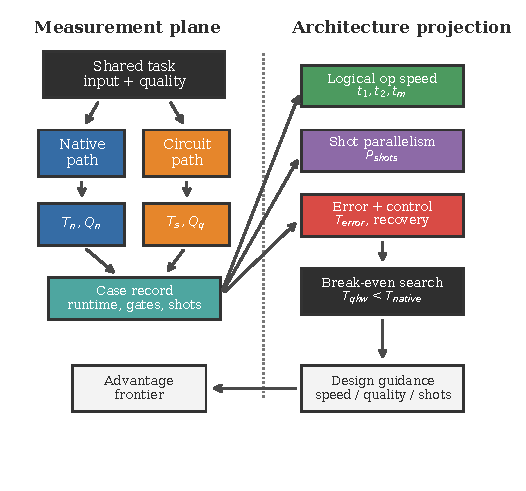
\includegraphics[width=\linewidth]{figures/design_overview.pdf}
    \Description{Block diagram of QSupremacy with shared workload control, native path execution, quantum path execution, measurement logging, and supremacy threshold analysis.}
    \caption{Architecture and procedure of \SystemName.}
    \label{fig:design-overview}
\end{figure}

\subsection{Overall Procedure}

Figure~\ref{fig:design-overview} shows the overall procedure. \SystemName has two main phases: \textit{Measurement} and \textit{Supremacy Analysis}.

\noindent\textbf{Measurement.}
When an experiment starts, \SystemName reads the workload configuration. The configuration includes the dataset, train/test split, feature dimension, model type, circuit type, shots, and target quality. \SystemName then runs the native path and the quantum-circuit path using the same input data. This prevents unfair comparisons caused by different preprocessing or different quality targets.

\noindent\textbf{Config Record.}
Before any path is executed, \SystemName materializes a single configuration record. This record is the logical owner of the experiment. It stores the workload family, instance ID, random seed, feature transform, native candidates, quantum circuit family, circuit depth, shot setting, and quality metric. The native and quantum paths do not choose these values independently. They receive the same record and append path-specific measurements to it. This mirrors the task-oriented style in the previous papers: the system first creates a stable representation of the work, then later components operate on that representation.

\noindent\textbf{Supremacy Analysis.}
After measurement, \SystemName reads the circuit metadata and runtime breakdown. It extracts the number of qubits, circuit depth, one-qubit gates, two-qubit gates, shots, and optimizer iterations. Using this information, \SystemName computes the quantum hardware speed required to make the projected quantum path faster than the measured native path.

\noindent\textbf{Failure Handling.}
\SystemName treats failed paths as measurement results rather than silently dropping them. If a native candidate fails, the record keeps the error and continues with other native candidates. If a quantum path fails, the record keeps the circuit metadata available up to the failure point and marks the case as non-advantaged. This rule is important for large sweeps because feasibility is part of the systems question. A workload that only succeeds after removing difficult cases would overstate the advantage frontier.

\subsection{Shared Workload Control}

\noindent\textbf{Dataset Control.}
\SystemName first fixes the workload. The first full workload is \texttt{sklearn digits}. \SystemName uses a fixed train/test split and applies PCA to 4, 8, 12, and 16 dimensions. The same reduced features are used by every native and quantum model.

\noindent\textbf{Instance Identity.}
Each measured case receives a deterministic identity. For ML, the identity includes the class pair, sample count, PCA dimension, circuit depth, and seed. For chemistry, it includes the molecule, basis, active-space setting, and circuit layer count. For optimization, it includes the graph family, graph size, seed, and QAOA layer count. For simulation, it includes the Hamiltonian model, number of qubits, evolution time, and approximation setting. This identity is used in filenames, JSON records, summaries, and paper figures. As a result, a figure bar can be traced back to the exact raw case that produced it.

\noindent\textbf{Application Control.}
\SystemName then extends the same rule to practical workloads. For drug discovery, the native path may be a classical molecular simulation or learned surrogate, while the quantum path may be a VQE-style molecular energy circuit. For optimization, the native path may be a mixed-integer, local-search, or GPU heuristic baseline, while the quantum path may be a QAOA-style circuit. For simulation, the native path may be a classical numerical solver, while the quantum path may be a Hamiltonian simulation circuit. In every case, \SystemName keeps the task, input instance, output metric, and quality target fixed.

\noindent\textbf{Quality Control.}
\SystemName defines the target quality before execution. The target can be a fixed accuracy threshold or a time-to-best-quality curve. This is important because a quantum path with lower accuracy cannot be claimed faster than a native path with higher accuracy.

\noindent\textbf{Quality Normalization.}
Different application families expose different quality values, so \SystemName stores both the native metric and a normalized gap. For classification, the gap is based on accuracy. For chemistry, it is based on energy error relative to the native reference. For optimization, it is based on objective gap. For simulation, it is based on state or observable error. The normalized gap lets the threshold analysis ask a common question across families: how much of the quality gap must future quantum hardware and algorithms recover before runtime speed becomes relevant?

\noindent\textbf{Why This Matters.}
Without shared workload control, the comparison becomes ambiguous. A native model may use a different feature dimension or a different split from the quantum model. \SystemName avoids this by making the workload controller the first step in the pipeline.

\subsection{Application Path Execution}

\subsubsection{Native Path Execution}

\noindent\textbf{Classical Baselines.}
The native path executes the best available non-quantum implementation for the same input. For ML, \SystemName supports softmax regression, MLP, linear ridge classification, RBF kernel ridge classification, k-nearest neighbors, and nearest-centroid baselines without requiring an external ML package. For chemistry, the native path computes molecular energy from the same Hamiltonian by exact dense diagonalization and, in the strengthened implementation, sparse Lanczos/eigensolver baselines for Pauli Hamiltonians. For optimization, \SystemName records exact enumeration when feasible and also greedy, local-search, and simulated-annealing baselines. For scientific simulation, the native path includes dense exact time evolution and a sparse Krylov-style evolution baseline. The native time used in the threshold is the fastest implemented model that reaches the best native quality within a small tolerance. This rule prevents a weak or low-quality native model from making the quantum path look artificially competitive.

\noindent\textbf{Runtime Breakdown.}
\SystemName records preprocessing time, training time, inference time, and total time. It also records accuracy and model metadata. These values define $T_{\mathrm{native}}$, which is the target that the projected quantum hardware path must beat.

\noindent\textbf{Baseline Selection Rule.}
The native path may produce several valid answers for one case. \SystemName first removes candidates that do not meet the family-specific quality rule. Among the remaining candidates, it selects the fastest one as the native baseline. If no native candidate reaches the quality target, the best-quality native candidate is still recorded, but the case is marked so that the threshold analysis does not create an artificial win. This selection rule is deliberately conservative: adding a stronger native method can only make the quantum threshold harder, not easier.

\subsubsection{Quantum Kernel Path}

\noindent\textbf{Feature Map Execution.}
The quantum kernel path maps each PCA feature vector into a quantum feature map. \cuQuantum simulates the circuit and produces state or observable data for kernel entries. A classical classifier then consumes the kernel matrix.

\noindent\textbf{Cost Breakdown.}
\SystemName records encoding time, circuit construction time, \cuQuantum execution time, kernel matrix construction time, and classifier-head time. This path is useful because it separates circuit execution cost from trainable quantum-parameter optimization.

\noindent\textbf{Expected Bottleneck.}
The kernel path can become expensive because the kernel matrix grows with the number of samples. Therefore, \SystemName must report both sample scaling and feature-dimension scaling.

\noindent\textbf{Kernel Accounting Rule.}
The kernel path is counted at the application level, not only at the circuit-kernel level. \SystemName records how many pairwise circuit evaluations are required, how many are actually executed, whether symmetry is used, and how the resulting matrix is consumed by the classifier. This matters because a circuit that is fast for one encoded sample can still be expensive after all sample pairs are evaluated. The design therefore exposes the sample-count multiplier instead of hiding it inside one aggregate runtime.

\subsubsection{QNN/VQC Path}

\noindent\textbf{Parameterized Circuit Execution.}
The QNN/VQC path maps the same PCA features into a parameterized quantum circuit. It then updates trainable parameters through a classical optimizer. Each optimizer step can require many circuit evaluations.

\noindent\textbf{Cost Breakdown.}
\SystemName records ansatz type, depth, gate count, number of parameters, optimizer iterations, observable extraction time, and accuracy. This path is expected to be more expensive than the quantum kernel path because training repeatedly evaluates the circuit.

\noindent\textbf{Why This Matters.}
QNN/VQC models are often discussed as quantum machine-learning candidates. However, their systems cost is easy to underestimate. \SystemName makes the repeated circuit evaluations visible.

\noindent\textbf{Optimizer Rule.}
For variational paths, \SystemName records the outer-loop optimizer separately from circuit execution. The record includes the number of parameter vectors, the number of observables, the number of shots per evaluation, and the measured time spent outside \cuQuantum. This separation is needed because future quantum hardware can reduce circuit execution time without removing the classical optimizer loop. If the optimizer or data movement dominates, the projected hardware speedup has limited effect.

\subsection{Measurement and Threshold Analysis}

\noindent\textbf{JSON Record.}
Every run emits a JSON record. The record includes dataset metadata, model metadata, runtime breakdowns, accuracy, circuit qubits, circuit depth, gate counts, shots, GPU metadata, and Slurm metadata where available.

\noindent\textbf{Summary Path.}
\SystemName keeps raw case records separate from derived summaries. A sweep first writes one JSON object per case or per task shard. A summarizer then validates expected case counts, merges shards, computes medians and quantiles, and writes CSV/JSON summaries used by the figures. The paper audit reads these summaries and checks that the claims in the manuscript match the stored values. This design follows the same spirit as prior systems papers: the evaluation does not depend on hand-copied numbers.

\noindent\textbf{Allocation Accounting.}
\SystemName separates login-node smoke tests from Slurm performance runs. Login-node tests are only for correctness. Slurm runs must record elapsed time, queue time, requested walltime, allocated GPUs, and charged node-hours. This prevents short sanity checks from being mistaken for valid performance experiments.

\subsubsection{Threshold Analysis}

\noindent\textbf{Execution Model.}
Given circuit metadata, \SystemName estimates projected quantum execution time:

\begin{align}
T_{\mathrm{execute}} =
\frac{N_s(D_1t_1 + D_2t_2 + D_mt_m)}
{P_{\mathrm{shots}}}
+ T_{\mathrm{error}},
\end{align}

where $N_s$ is the shot count, $D_1$ and $D_2$ are one- and two-qubit gate depths, $D_m$ is measurement depth, $t_1$, $t_2$, and $t_m$ are logical operation times, and $P_{\mathrm{shots}}$ is shot-level parallelism.

\noindent\textbf{Break-even Search.}
\SystemName inverts the model. Instead of assuming a quantum speedup, it asks what logical gate time, shot throughput, and error overhead are needed for:

\begin{align}
T_{\mathrm{qhw}} < T_{\mathrm{native}}.
\end{align}

This gives a hardware requirement rather than a vague claim of supremacy.

\noindent\textbf{Advantage Frontier.}
\SystemName does not reduce the result to one speedup number. It sweeps hardware assumptions and reports the feasible region where the projected quantum path beats the native path at the same quality. This region is the advantage frontier. If no reasonable region exists, the workload is classified by the limiting factor: quality, encoding, shots, error overhead, or native baseline strength.

\noindent\textbf{Frontier Classification.}
After the sweep, each case is assigned a primary limiting factor. A case is speed-limited when quality is close enough but the required runtime improvement is large. It is quality-limited when even aggressive speedup does not help unless the output gap closes. It is encoding- or shot-limited when non-kernel overhead dominates the projection. It is native-dominated when a strong native baseline makes the required improvement much larger than the quantum path can plausibly recover. This classification turns the frontier into a diagnostic result instead of only a plot.

\subsection{Advantage Claim Checklist}

A practical quantum-advantage claim should pass a small set of systems checks before it is treated as meaningful. Table~\ref{tab:claim-checklist} lists the checks used by \SystemName. The checklist is intentionally strict because a weak native baseline, a different input instance, or a lower-quality quantum output can all create a false impression of advantage.

\begin{table}[t]
\caption{Checklist for a practical quantum-advantage claim.}
\centering
\small
\resizebox{\columnwidth}{!}{%
\begin{tabular}{lll}
\toprule
\textbf{Check} & \textbf{Question} & \textbf{\SystemName evidence} \\
\midrule
Same task & Are native and quantum paths solving the same input? & Shared workload config \\
Same quality & Does the quantum path meet the native target? & Accuracy, energy, objective, observable gap \\
Strong native & Is the native path the fastest valid baseline? & Baseline selection rule \\
End-to-end cost & Are encoding, execution, measurement, and postprocess included? & Runtime breakdown and metadata \\
Hardware projection & What future quantum speed is required? & Required speedup and frontier \\
Error/shot overhead & Could shots or error correction erase speedup? & Projection parameters and sensitivity \\
Repeatability & Can the result be regenerated on the system? & Slurm scripts, summaries, accounting \\
\bottomrule
\end{tabular}
}
\label{tab:claim-checklist}
\end{table}

\subsection{Workload Suite}

Table~\ref{tab:workload-suite} shows the measured workload suite. The digits workload is the controlled calibration case. The practical suite covers the application families that motivate many real-world quantum-computing claims.

\begin{table}[t]
\caption{Measured workload suite.}
\centering
\small
\resizebox{\columnwidth}{!}{%
\begin{tabular}{llll}
\toprule
\textbf{Family} & \textbf{Native path} & \textbf{Quantum path} & \textbf{Quality target} \\
\midrule
ML classification & Logistic/MLP/SVM & Kernel, QNN/VQC & Accuracy, loss \\
Drug discovery & Classical energy/surrogate & VQE energy circuit & Energy error, rank quality \\
Optimization & MILP/heuristic/GPU search & QAOA circuit & Objective gap \\
Scientific simulation & Classical solver & Hamiltonian simulation & State/error metric \\
\bottomrule
\end{tabular}
}
\label{tab:workload-suite}
\end{table}

\section{Evaluation}

The evaluation follows the inversion order in Figure~\ref{fig:design-overview}. We first establish a deployment-facing native frontier, then determine which circuit records satisfy application quality, and only then derive logical and physical architecture targets. Perlmutter is the evidence engine throughout; its GPU time is never substituted for QPU time.

\subsection{Evaluation Setup and Contracts}

\noindent\textbf{Platform and evidence units.}
Experiments run on \LeadershipSystem GPU nodes, each with four NVIDIA A100 GPUs. The controlled corpus contains 3,552 records: 2,048 ML, 224 Chem., 768 Opt., and 512 Sim. records. These records cover 222 structural configurations and 16 distinct seeds per configuration. A structural configuration fixes the input and algorithm settings; a seed within that configuration is an independent observation, not a repeated timing trial. We report hierarchical-bootstrap 95\% intervals over configurations and seeds using 2,000 resamples, and macro-averages weight the four families equally. Warmup-separated stability trials and all raw failures are stored separately.

This distinction changes the reported uncertainty. The workload-balanced noiseless quality-pass fraction is 17.9\% with a 95\% interval of 11.2--24.8\%, rather than a raw-record average dominated by ML. The geometric mean of the four family-median simulator/native ratios is 19,329$\times$ (18,108--26,829$\times$). Twelve warmup-separated timing trials, three per family, have a maximum quantum-runtime coefficient of variation of 4.0\%. Capacity probes and deterministic design scenarios are reported as bounds rather than assigned sampling confidence.

Table~\ref{tab:evaluation-setup} defines the paired application contract. A quality pass requires the quantum path to remain within the listed natural-unit tolerance of the native output. The main corpus is exact/noiseless and exposes representation or approximation error. A separate direct experiment selects 68 source records and samples each at $10^3$, $10^4$, and $10^5$ shots with 12 independent replicates. Hardware eligibility additionally requires at least 0.9 pass probability, a measurement trace for the same record, and coverage of the complete application loop.

\begin{figure}[t]
\centering
\begin{subfigure}[t]{\linewidth}
\centering
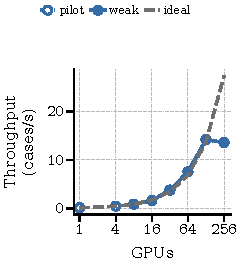
\includegraphics[width=0.98\linewidth]{figures/weak_scaling.pdf}
\caption{Weak evidence generation.}
\label{fig:evidence-weak-scaling}
\end{subfigure}
\vspace{-0.25em}
\begin{subfigure}[t]{\linewidth}
\centering
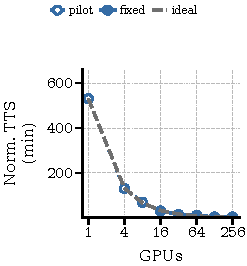
\includegraphics[width=0.98\linewidth]{figures/strong_scaling.pdf}
\caption{Fixed 7,104-record sweep.}
\label{fig:evidence-strong-scaling}
\end{subfigure}
\Description{Perlmutter weak and fixed-work scaling for independent application-record generation from one to 256 GPUs. Hollow markers distinguish context or split-array anchors from direct regular runs.}
\caption{Perlmutter evidence-generation scaling. Actual and ideal lines compare completed corpus runs; the hollow 1-GPU point is a split-array anchor. Timeout-censored 4/8/16-GPU attempts are not plotted as fixed-work completions.}
\label{fig:evidence-scaling}
\end{figure}

\begin{figure*}[!t]
\centering
\begin{subfigure}[t]{0.315\linewidth}
    \centering
    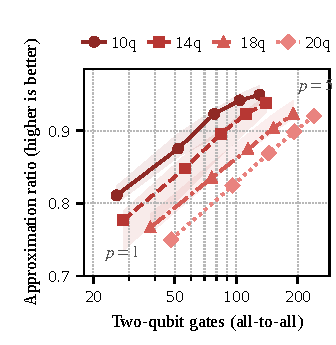
\includegraphics[width=\linewidth]{figures/opt_qaoa_quality_proxy.pdf}
    \caption{Opt. depth--quality cost.}
    \label{fig:opt-qaoa-quality-proxy}
\end{subfigure}
\hfill
\begin{subfigure}[t]{0.315\linewidth}
    \centering
    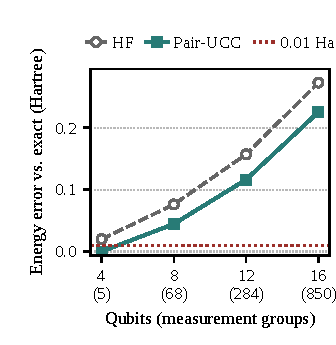
\includegraphics[width=\linewidth]{figures/chem_vqe_quality_cost_proxy.pdf}
    \caption{Chem. active-space closure.}
    \label{fig:chem-vqe-quality-proxy}
\end{subfigure}
\hfill
\begin{subfigure}[t]{0.315\linewidth}
    \centering
    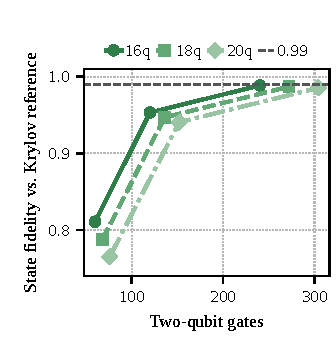
\includegraphics[width=\linewidth]{figures/sim_quality_cost_proxy.pdf}
    \caption{Sim. Trotter quality cost.}
    \label{fig:sim-quality-cost-proxy}
\end{subfigure}
\Description{Measured quality-cost curves for QAOA, VQE-style pair-UCC, and Trotterized Hamiltonian simulation.}
\caption{Quality recovery consumes circuit work. Opt. depth improves approximation ratio while multiplying routed two-qubit gates; Chem. measurement groups grow while larger active spaces remain outside chemical accuracy; Sim. state fidelity improves with Trotter depth.}
\label{fig:large-proxy-quality-cost}
\end{figure*}

\begin{table}[t]
\caption{Same-input application contracts. Deployment-facing native cases strengthen the frontier but do not alter controlled-corpus quality.}
\centering
\footnotesize
\setlength{\tabcolsep}{2.6pt}
\renewcommand{\arraystretch}{1.08}
\begin{tabular}{p{0.12\columnwidth}p{0.36\columnwidth}p{0.40\columnwidth}}
\toprule
\textbf{Family} & \textbf{Native path} & \textbf{Circuit path and quality gate} \\
\midrule
ML & scikit classifiers; matched Pool-108; A100 ResNet-18 & QKernel, QNN/VQC, or QFeature; accuracy loss $\leq0.02$ \\
Chem. & dense/sparse eigensolver; FCI/CASCI; CCSD(T) & VQE-style preparation and Pauli energy; error $\leq0.01$ Ha \\
Opt. & exact, local search, annealing, or MILP & QAOA sampling; approximation-ratio loss $\leq0.02$ \\
Sim. & dense or matrix-free Krylov evolution & Trotter circuit and terminal observable; error $\leq0.01$ \\
\bottomrule
\end{tabular}
\label{tab:evaluation-setup}
\end{table}

\noindent\textbf{Scale and provenance.}
Figure~\ref{fig:evidence-scaling} verifies that Perlmutter increases the rate at which paired application records are built. With about 28 records per GPU, aggregate throughput reaches 12.3 records/s on 256 GPUs. For the completed direct 7,104-record runs, elapsed time falls from 2,894~s on 32 GPUs to 418~s on 256 GPUs, a 6.9$\times$ speedup. The hollow 1-GPU point is a split-array anchor. Separate 4/8/16-GPU attempts reached 4,298/5,794/7,092 records before their 8/5/3-hour limits; they are censored and never extrapolated into measured completion times. This is case-level parallelism, not distributed execution of one circuit.

We separate semantic closure from state-vector capacity. The controlled applications remain at 4--20 qubits so that their native answer, circuit output, and quality gap can be checked exactly. Separate completed probes hold a 36-qubit, 0.5-TiB state on 64 GPUs; a 38-qubit, 2.0-TiB state on 128 GPUs; and a 40-qubit, 8.0-TiB state on 256 GPUs. The corresponding shards are 8, 16, and 32~GiB/GPU. Median local-gate time remains within 0.614--0.807~s as aggregate state grows by 16$\times$, while the 38-qubit maximum exposes a 29.888-s straggler. Each rank transforms only its local shard, so these runs establish storage reach and process coverage, not a complete cross-rank application or QPU scaling.

The physical analysis instead consumes gates, angles, shots, dependency-ready work, quality, and native deadlines from the paired records. All 224 Chem. records have compiled measurement groups, 3,040 ML/Chem./Opt. records have source-audited static loops, and all 512 Sim. records have one terminal circuit. No adaptive optimizer or mid-circuit trace is inferred. Keeping the capacity probes separate prevents a large stored vector from being mistaken for large-scale application-quality closure.

\subsection{Deployment-Facing Native Frontier}

The controlled suite is intentionally small enough to close input, circuit, and exact quality. We therefore add deployment-facing native paths before projecting hardware. A stronger native implementation only shortens $T_{\mathrm{native}}$ and moves the break-even boundary outward; it cannot manufacture a favorable quantum result.

\noindent\textbf{ML representation.}
Figure~\ref{fig:ml-cifar-matched} compares three paths on the same CIFAR-10 50,000/10,000 split. A one-A100 ResNet-18 trained for 10 epochs with AMP/TF32 takes 56.5~s and reaches 81.85\% accuracy. QFeature uploads 4,096 amplitudes to 12 qubits, applies three entangling layers, extracts 108 observables, and trains a ridge head; it takes 115.16~s and reaches 33.60\%. Pool-108 uses the same feature count and ridge head but fixed spatial pooling, taking 2.45~s and reaching 40.28\%. Thus the circuit representation is 46.97$\times$ slower and 6.68 points less accurate than its matched control before QEC, shots, or generic state preparation. Faster logical gates cannot close this representation gap.

\begin{figure}[H]
\centering
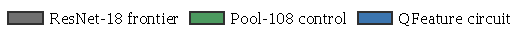
\includegraphics[width=0.96\linewidth]{figures/ml_cifar10_legend.pdf}
\vspace{-0.35em}
\begin{subfigure}[t]{0.48\linewidth}
\centering
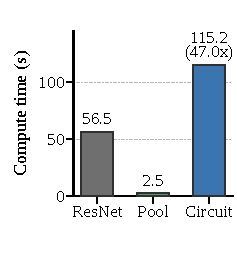
\includegraphics[width=\linewidth]{figures/ml_cifar10_runtime.pdf}
\caption{Measured compute time.}
\label{fig:ml-cifar-runtime}
\end{subfigure}
\hfill
\begin{subfigure}[t]{0.48\linewidth}
\centering
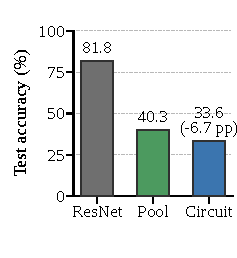
\includegraphics[width=\linewidth]{figures/ml_cifar10_accuracy.pdf}
\caption{Test accuracy.}
\label{fig:ml-cifar-accuracy}
\end{subfigure}
\Description{Matched CIFAR-10 comparison of runtime and accuracy for ResNet-18, fixed spatial pooling, and a cuQuantum feature circuit.}
\caption{Matched CIFAR-10 outcomes. Pool-108 and QFeature expose 108 features to the same ridge head; direct annotations show that QFeature is 47.0$\times$ slower and 6.7 points less accurate than this matched control. ResNet-18 provides the deployment-facing native quality frontier.}
\label{fig:ml-cifar-matched}
\end{figure}

\noindent\textbf{Quality costs beyond ML.}
Figure~\ref{fig:large-proxy-quality-cost} measures the work needed to recover quality rather than assuming that recovery is free. For weighted MaxCut, increasing directly optimized QAOA from $p=1$ to 5 raises the median 10/14/18-qubit approximation ratio from 0.785 to 0.938, but raises all-to-all 2Q work from 28 to 140 gates; line routing expands it by 2.15--2.56$\times$. The 20-qubit $p=5$ case reaches 0.920 with 240 all-to-all or 898 line-routed 2Q gates. Native 50--100-node local search and annealing reach median 0.998 and 1.000 of the best observed objective.

For Chem., nested 4/8/12/16-qubit H$_8$ active spaces compare pair-UCC with exact FCI. Only the 4-qubit space closes 0.01~Ha; best errors are below $10^{-8}$, 0.04465, 0.11637, and 0.22547~Ha while qubit-wise-commuting groups grow from 5 to 850. Deployment N$_2$/H$_2$O CCSD(T) instances map to 120/184 spin-orbital qubits, but do not have a matched large-space VQE-quality closure and are not assigned a physical target. For Sim., 20-qubit Trotter fidelity rises from 0.765 to 0.985 at 4/8/16 steps while 2Q gates rise from 76 to 304; the native matrix-free Krylov reference takes 0.56--20.56~s at 16--20 qubits with norm error below $6\times10^{-14}$. These results identify representation, ansatz/search, and approximation order as first-class architecture inputs rather than NISQ-noise artifacts.

Figure~\ref{fig:roofline-native-stress} applies an adversarial native stress using the A100 tensor-core/HBM peaks and a 10-$\mu$s launch floor under the Roofline method~\cite{williams2009roofline}. It shortens the implemented native deadline by a median 209$\times$/17$\times$/2.4$\times$/208$\times$ for ML/Chem./Opt./Sim. The stress is an unattainable lower bound, not a measured implementation or a SOTA claim. Its role is to test direction: replacing any executed native path with a more optimized one can only make the quantum boundary harder. We retain the measured deadline in subsequent projections, so their runtime targets remain optimistic with respect to this stress.

\begin{figure}[H]
\centering
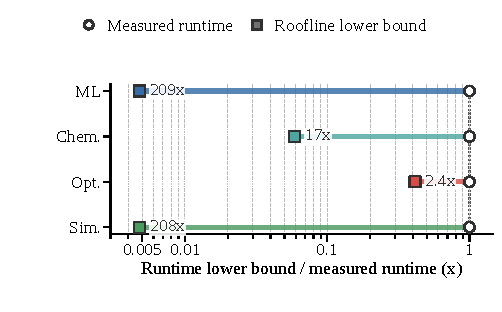
\includegraphics[width=0.96\linewidth]{figures/roofline_deadline_shrink.pdf}
\Description{A dumbbell plot connects each measured native runtime to an A100 tensor-core and HBM roofline lower bound with a ten-microsecond launch floor.}
\caption{Adversarial native-runtime stress. Circles normalize each measured family median to 1; squares show the peak/HBM lower bound. Moving left gives the circuit path less time to beat native HPC; the span is not measured application speedup.}
\label{fig:roofline-native-stress}
\end{figure}

\begin{observationbox}
\noindent\textbf{Observation 1:} A stronger native implementation moves the advantage boundary outward, while better circuit quality adds gates, measurements, or search work. QPU targets must therefore use the paired native deadline and charge the measured cost of quality recovery.
\end{observationbox}
\FloatBarrier

\subsection{Quality-Qualified Application Boundary}

Hardware speed matters only after the circuit output is useful. Figure~\ref{fig:quality-gates} therefore applies the quality gate before any hardware projection. In the full noiseless corpus, no ML or Opt. record passes; 48/224 Chem. and 256/512 Sim. records pass. The 95\% hierarchical-bootstrap intervals are [0,0], [0,0], [0,0.429], and [0.344,0.688], respectively. Halving or doubling each tolerance preserves this ordering.

\begin{figure}[t]
\centering
\begin{subfigure}[t]{0.47\linewidth}
\centering
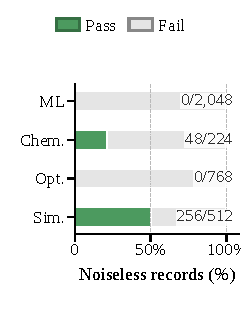
\includegraphics[width=\linewidth]{figures/quality_noiseless_gate.pdf}
\caption{Full noiseless corpus.}
\label{fig:quality-noiseless}
\end{subfigure}
\hfill
\begin{subfigure}[t]{0.49\linewidth}
\centering
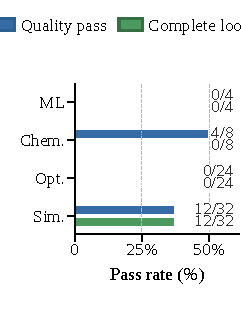
\includegraphics[width=\linewidth]{figures/quality_finite_shot_gate.pdf}
\caption{Direct finite-shot cases.}
\label{fig:quality-finite-shot}
\end{subfigure}
\Description{Quality-pass and failure fractions for the full noiseless corpus, followed by quality-pass and complete-application-loop fractions for the direct ten-thousand-shot experiment.}
\caption{Quality eligibility precedes hardware targeting. The 3,552-record noiseless corpus yields 304 quality passes. A separate 68-record direct audit at $10^4$ shots yields 16 quality passes, but only 12 Sim. records cover the complete same-record application loop and become physical targets. Counts beside every bar retain the panel-specific denominator.}
\label{fig:quality-gates}
\end{figure}

At $10^4$ shots, ML passes 0/4, Chem. 4/8, Opt. 0/24, and Sim. 12/32. The Chem. passes sample one fixed parameter set and do not include VQE optimization. ML changes to a measurable Z/ZZ feature map but still misses the accuracy bound. Opt. samples fixed QAOA parameters and omits the outer search. These are algorithm and loop gaps, not NISQ noise: the source corpus is noiseless. Only the 12 Sim. cases at the declared $10^4$-shot contract are same-record, full-loop, quality-qualified hardware targets. Physical numbers for every other family are explicitly conditional lower bounds. At $10^3$ shots no case passes; at $10^5$, Chem. remains 4/8 and Sim. rises to 16/32.

The split follows application-loop structure. ML and Opt. lose quality before hardware timing begins, while the passing Chem. outputs still omit the optimizer that would repeatedly request energies. Sim. has one terminal observable and no hybrid outer loop, so its passing records can close the full application contract. The first architecture action is therefore family-specific: improve representation or search for ML/Opt., close the measured VQE loop for Chem., and only then optimize QPU resources for eligible Sim.

\begin{observationbox}
\noindent\textbf{Observation 2:} Faster gates cannot rescue an output that fails the application contract. ML, Chem., and Opt. first need better representations, ansatzes, or searches; only the 12 full-loop Sim. records support physical hardware targets.
\end{observationbox}
\FloatBarrier

\subsection{Trace-Aware Logical Lower Bound}

The next test gives the QPU free magic states and asks whether logical execution alone can beat native HPC. It removes simulator wall time and factory latency, but keeps direct $10^4$ shots, case-level reliability, logical work, useful-lane limits, decoder reaction, and host-visible rounds. Figure~\ref{fig:trace-logical-lower-bound} shows only the 12 Sim. cases that passed the full-loop gate in Figure~\ref{fig:quality-gates}.

\begin{figure}[t]
\centering
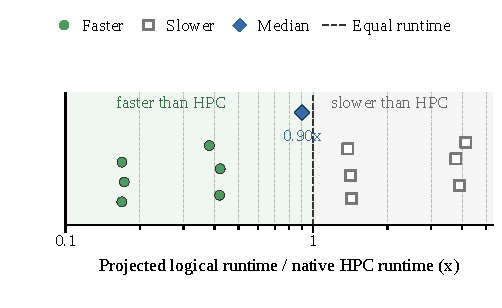
\includegraphics[width=0.98\linewidth]{figures/trace_aware_logical_lower_bound.pdf}
\Description{Twelve quality-qualified simulation records plotted by projected logical runtime with free T-state generation relative to measured native-HPC runtime. Filled circles are faster than native HPC, open squares are slower, and a diamond marks the median.}
\caption{Logical-runtime lower bound with free T-state generation at $10^4$ shots. Each point is one eligible Sim. record; the dashed line marks equal native-HPC runtime and the diamond is the median.}
\label{fig:trace-logical-lower-bound}
\end{figure}

The eligible records span 0.170--3.891$\times$ native time from the 10th to 90th percentile. Their median is 0.903$\times$, and 6/12 beat native time. The schedule variants coincide because each record has one terminal circuit. For context, the same optimistic model gives conditional medians of 90.6$\times$ for ML, 526.2$\times$ for group-ready Chem., and 3,653.9$\times$ for Opt.; these are not hardware targets because they failed Figure~\ref{fig:quality-gates}. Removing Perlmutter simulation cost therefore does not guarantee advantage. Finite-shot logical work already blocks half of the eligible records.

This split is not a simulator constant. Each ratio combines that record's measured native time with its own logical work and direct shot count. The same workload family therefore falls on both sides of parity. An architecture must reduce useful logical work or execute independent shots concurrently without weakening the quality contract; a single average gate-speed claim cannot predict which records cross the boundary.

The lower bound is also an early rejection test for component proposals. All 12 records use only 4--7 logical qubits, yet their ratios span both sides of native parity; qubit count alone does not determine the result. A mechanism that changes T-state factories, movement, or decoder service cannot rescue an open-square record that is slower than native HPC, because those costs are already free or absent from this test. Such a record first needs a shorter logical schedule, more dependency-ready shot concurrency, or fewer shots at the same measured quality. For a filled-circle record that is already faster, those logical conditions are sufficient and the physical stack becomes the next question. The test therefore prevents a downstream component gain from being credited before the record reaches that component.

\begin{observationbox}
\noindent\textbf{Observation 3:} Even with free T states, only 6/12 eligible records beat native HPC. Their first useful target is lower logical and shot work, while the other six already have enough logical speed and expose the physical factory cost next.
\end{observationbox}
\FloatBarrier

\subsection{Reliability-Constrained Physical Diagnosis}

Figure~\ref{fig:ft-reliability-target} restores arbitrary-rotation synthesis and distillation for the 12 eligible records. Under a 1\% application-failure budget and physical error $10^{-3}$, the all-shots contract, aligned with QDK, selects distance 13--15 and 79--86 T states per arbitrary rotation. A sensitivity that allows a bounded number of failed shots selects distance 7--9 and 49--58 T states. Panel (a) exposes both resource settings rather than hiding them behind one global distance or T count. The compatible all-shots protocol uses 2,070 physical qubits per factory output path~\cite{azureestimator,rossselinger2016}.

\begin{figure}[t]
\centering
\begin{subfigure}[t]{\linewidth}
\centering
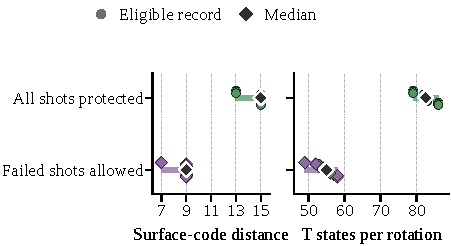
\includegraphics[width=0.96\linewidth]{figures/ft_contract_parameters.pdf}
\caption{Per-record error-correction settings.}
\label{fig:ft-contract-parameters}
\end{subfigure}
\vspace{-0.2em}
\begin{subfigure}[t]{\linewidth}
\centering
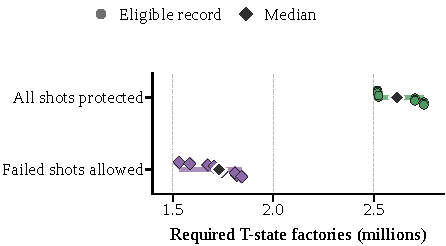
\includegraphics[width=0.96\linewidth]{figures/ft_reliability_target.pdf}
\caption{Parallel T-state factories required.}
\label{fig:ft-factory-crossover}
\end{subfigure}
\Description{Surface-code distance and T-state demand per eligible record, followed by the absolute number of parallel T-state factories required under an all-shots contract and a bounded failed-shot sensitivity.}
\caption{Reliability choices set physical cost. Points are the 12 eligible records and diamonds mark medians. (a) Protecting every shot requires larger codes and more T states per rotation than allowing a bounded failed-shot tail. (b) The two contracts require 1.53--2.75 million parallel T-state factories before T-state generation stops dominating. Failed-shot tolerance is a sensitivity, not the default.}
\label{fig:ft-reliability-target}
\end{figure}

The all-shots contract requires 2.52--2.75 million factories operating in parallel, equivalent to 39,351--42,961$\times$ the 64-factory baseline. Their protocol footprint is 5.21--5.69 billion factory qubits. This is a supply-equivalent target, not a floorplan. It is large because every arbitrary rotation is repeated over $10^4$ shots while the reliability budget tightens both T-state error and code distance. Allowing a bounded failed-shot tail reduces the target to 1.53--1.84 million factories, distance 7--9, and 49--58 T states per rotation, but does not change the first bottleneck. Decoder reaction combines 7.8~$\mu$s communication with 1/5/63~$\mu$s service envelopes~\cite{khalid2025reaction}; at 5~$\mu$s, median syndrome bandwidth is 3.09~Gb/s. Control becomes important later, after factory supply is no longer dominant.

Space gives the same diagnosis. Across the 12 eligible records, protected data occupies 1,352--3,150 physical qubits, while the compatible QDK factory protocols occupy 5.21--5.69 billion qubits at crossover. Mapping the same supply into LSQCA's 176-cell density envelope gives a separate 150--218-billion-qubit upper envelope; the two models are reported separately, not multiplied. At the 5-$\mu$s decoder point, reaction-time correction storage alone spans 2.56--3.71 billion qubits and the data-block syndrome stream spans 1.69--3.94~Gb/s. These values do not propose such a machine. They show that synthesized-rotation supply and its protected state dominate the data block before decoder or layout improvements can become first-order.

\begin{observationbox}
\noindent\textbf{Observation 4:} Fault tolerance reverses the favorable result with free T-state generation. The first physical target is not a slightly faster gate, but four to five orders of magnitude more useful T-state throughput; relaxed reliability reduces its size but not its identity.
\end{observationbox}
\FloatBarrier

\subsection{Joint Co-Design Sensitivity}

Improving one resource moves the bottleneck to another. We evaluate 384 deterministic scenarios across quality, shots, useful lanes, T count, reliability, physical error, factory supply, logical cycle, decoder service, native time, dependencies, and overlap. Figure~\ref{fig:joint-phase-map} keeps the all-shots contract and shows which 10$\times$ resource upgrade reduces runtime most for each of the 12 eligible records. Repeated cells with identical outcomes are collapsed.

Eligibility is recomputed inside each scenario rather than held at 12 by construction: changing shots or tolerance can move a record across the quality gate. Likewise, fixed 16- or 32-T rotation scenarios that violate the precision-derived synthesis budget are retained as invalid sensitivities but cannot support a physical target. The plotted slice fixes the declared $10^4$-shot quality contract, reliability-derived T count, 1\% application budget, and $10^{-3}$ physical error so that every transition is executable under one consistent contract.

The complete space-filling design contains 128 reliability-derived-T points in addition to invalid fixed-T stresses. Forty-one have no valid eligible modal target and remain unclassified rather than being forced into a hardware category. Of the remaining 87, 60 are factory-first, 13 shot-first, four logical-cycle-first, and ten already reach advantage. Supply explains the transition without assigning scenario probabilities: at 1--100$\times$ factory supply, 44/45 valid modal decisions are factory-first; at 10k$\times$, the valid modes split into 12 factory, eight shot, one cycle, and two advantage; at 50k$\times$, they split into four, five, three, and seven. Figure~\ref{fig:joint-phase-map} isolates the declared contract so the causal handoff is not hidden by quality and FT-invalid points.

\begin{figure}[t]
\centering
\begin{subfigure}[t]{\linewidth}
\centering
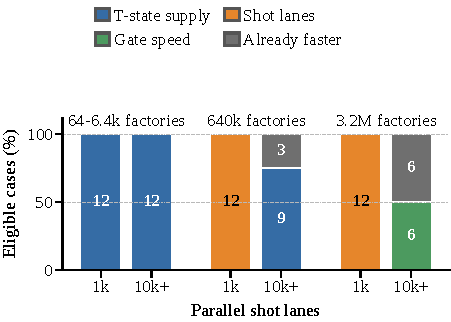
\includegraphics[width=0.96\linewidth]{figures/joint_bottleneck_phase_map.pdf}
\caption{Best next 10$\times$ resource upgrade.}
\label{fig:joint-first-target}
\end{subfigure}
\vspace{-0.2em}
\begin{subfigure}[t]{\linewidth}
\centering
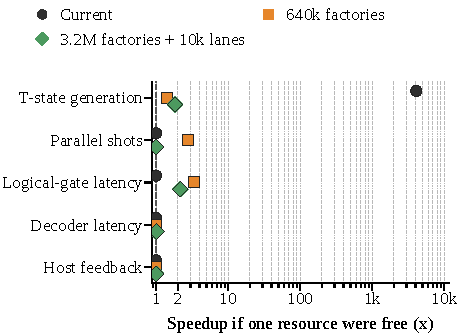
\includegraphics[width=0.96\linewidth]{figures/resource_removal_ceiling.pdf}
\caption{Maximum gain if one resource were free.}
\label{fig:joint-removal-ceiling}
\end{subfigure}
\Description{The resource whose tenfold improvement reduces runtime most and the maximum median speedup from removing one resource cost for twelve eligible simulation records.}
\caption{How the next useful upgrade changes. (a) Each colored segment counts records for which a 10$\times$ improvement to that resource reduces runtime most; ``already faster'' means projected runtime is below native HPC. Group headings give absolute T-state factory counts and ticks give parallel shot lanes. (b) Each marker is the median speedup if one resource cost becomes free; 1$\times$ means no useful leverage.}
\label{fig:joint-phase-map}
\end{figure}

At 1--100$\times$ factory supply, factory supply is first for every lane count. At $10^4\times$, 1,000 lanes makes shot parallelism first; with at least 10,000 lanes, three records reach advantage and nine remain factory-limited. At $5\times10^4\times$, 1,000 lanes is still shot-limited; at least 10,000 lanes leaves six advantaged and six logical-cycle-limited records. Thus the useful order is factory throughput, shot lanes, and then logical-cycle latency. Decoder and host latency do not become first in this slice.

Panel (b) separates the next 10$\times$ action from the maximum possible gain. At the current point, making T-state generation free gives a median 4,102$\times$ speedup, whereas making shot, gate-cycle, decoder, or host cost free gives at most 1.00024$\times$. With 640,000 factories and 1,000 lanes, the maximum gains from free shot and gate-cycle cost rise to 2.76$\times$ and 3.34$\times$; the next 10$\times$ test still selects shot lanes first. With 3.2 million factories and 10,000 lanes, gate-cycle cost has the largest remaining gain at 2.17$\times$, followed by T-state generation at 1.82$\times$, while decoder and host remain below 1.01$\times$. The distinction prevents a large asymptotic gain from displacing the resource that gives the next realizable improvement.

Each bar segment is a design decision, not a probability assigned to a future technology. ``T-state supply'' means that a 10$\times$ supply improvement gives the largest compatible runtime reduction for that record; ``already faster'' means the complete quality-qualified runtime is below native HPC. The transition across columns is therefore causal: adding factories alone eventually exposes serialized shots, and adding useful lanes then exposes logical-gate latency. Collapsing identical settings keeps the figure focused on these transitions rather than repeated parameter combinations.

The framework can also test a published mechanism without borrowing its reported mean speedup. Figure~\ref{fig:lsqca-matched-replacement} inserts LSQCA point-SAM core cells and matched load/store events into the $5\times10^4$-factory, 10,000-lane point while holding all other terms fixed~\cite{lsqca2025}. These 4--7-qubit circuits are below point-SAM's seven-qubit area break-even, so none gains core area. The lower and upper movement envelopes increase median runtime by 3.12$\times$ and 5.23$\times$ and remove all six runtime passes. This does not judge LSQCA at its intended scale; it shows that a mechanism must be matched to workload events.

\begin{figure}[t]
\centering
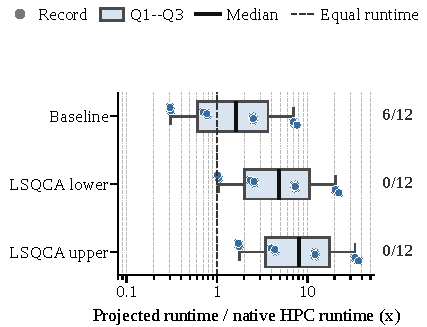
\includegraphics[width=0.98\linewidth]{figures/lsqca_matched_replacement.pdf}
\Description{Twelve runtime ratios before and after lower and upper matched LSQCA point-SAM movement, with medians and percentile ranges.}
\caption{Matched-event LSQCA replacement. Points are the 12 eligible records; boxes span Q1--Q3, center lines mark medians, whiskers span p10--p90, and the dashed line marks equal native-HPC runtime. Right labels count runtime passes. Only core cells and movement change.}
\label{fig:lsqca-matched-replacement}
\end{figure}

A BOSS-compatible graph envelope also bounds QCCD routing without claiming a device simulation~\cite{boss2025}. Chem. adds zero locality-first shuttles and at most 24 at the p90 congestion bound; Opt. adds median 7 and 35.5, respectively. Because both families fail the quality gate, these remain conditional routing bounds.

The first target also depends on physical modality. Figure~\ref{fig:sim-modality-pivot} re-prices the same 12 eligible Sim. demands under the all-shots surface-code path and two literature-calibrated native-rotation envelopes. At the measured surface-code point, the median projection is 36,212$\times$ slower than native and T-state generation accounts for 99.98\% of execution time, consistent with the 4,102$\times$ maximum gain when that cost is removed. Replacing synthesized rotations with the neutral-atom envelope moves 98.3\% of time to readout/reuse; a 10$\times$ readout improvement gives an 8.71$\times$ end-to-end gain. The QCCD envelope instead assigns 79.6\% to two-qubit gates and 11.8\% to readout; a 10$\times$ two-qubit-gate improvement gives 3.52$\times$. Thus the inversion does not prescribe one universal QPU. It identifies T-state generation for synthesized surface-code execution, readout/reuse for the zoned native-rotation envelope, and entangling gates for the QCCD envelope.

\begin{figure}[t]
\centering
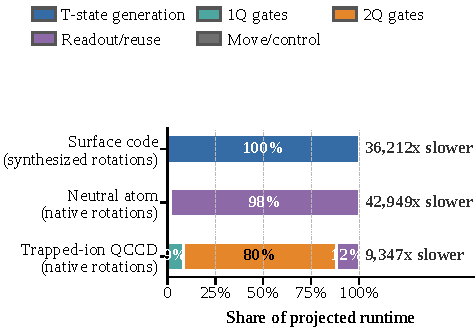
\includegraphics[width=0.98\linewidth]{figures/sim_hardware_modality_pivot.pdf}
\Description{Normalized execution shares for the same twelve quality-qualified simulation records under synthesized surface-code execution and two literature-calibrated native-rotation timing envelopes, with absolute slowdown versus native beside each row.}
\caption{Where projected time goes under three QPU approaches. Each row is normalized to its own runtime, and the right label reports the absolute slowdown versus native HPC. The surface-code row uses the all-shots contract; native-rotation rows are execution-only counterfactuals calibrated from neutral-atom and QCCD reports~\cite{bluvstein2026faulttolerant,boss2025}, without hardware noise or a fault-tolerance claim.}
\label{fig:sim-modality-pivot}
\end{figure}

Removing factories is therefore necessary but not sufficient. The neutral-atom and QCCD envelopes remain median 42,949$\times$ and 9,347$\times$ slower than the paired native deadlines because $10^4$ measured shots repeatedly pay readout or gate time. These ratios are not present-device benchmarks: count-based intra-circuit parallelism is optimistic, the neutral-atom control attachment is a lower bound, and the QCCD path prices extra routed gates as recooling rather than running a full transport schedule. Their value is architectural: they show which measured event a specialized accelerator must remove next, while preserving the same finite-shot quality and native deadline.

Resources absent from Figure~\ref{fig:joint-phase-map} are also informative. Decoder, host/control, and matched layout work have low marginal value while rotation supply or shot serialization remains upstream. This is not a claim that they never matter. It says their application-level value must be re-evaluated after the earlier crossover, using the dependency and movement events of the same record. Figure~\ref{fig:lsqca-matched-replacement} demonstrates the converse: introducing a layout mechanism too early can add enough movement to erase every favorable case.

\begin{observationbox}
\noindent\textbf{Observation 5:} QArchGauge returns an ordered build decision, not one universal bottleneck. ML and Opt. stop at output quality, and Chem. stops at full-loop closure; none yet justifies a physical-QPU target. For the 12 eligible Sim. records, the all-shots surface-code path first needs less synthesized-rotation demand or 2.52--2.75 million parallel T-state factories. Between 640,000 and 3.2 million factories, at least 10,000 parallel shot lanes prevent sampling serialization. After both improve, logical-gate latency becomes first for the remaining six records. Decoder, control, and layout are not first at the measured point, and charging matched LSQCA movement removes all six otherwise favorable cases. The measured build order is therefore algorithm/loop, T-state generation, parallel shots, and logical-gate latency; a component should move forward only when its matched events become first.
\end{observationbox}
\FloatBarrier

\section{Related Work}

\noindent\textbf{Quantum Simulation and NISQ Systems.}
Computer architecture uses measurement and modeling to study immature systems~\cite{skadron2003challenges}; \SystemName applies that discipline to quantum systems. ScaleQsim, AURORA-Q, and \cuQuantum improve state-vector simulation through distribution, GPUs, tiered memory, asynchronous movement, and optimized primitives~\cite{scaleqsim,auroraq,cuquantum}; NISQ studies show current-device limits~\cite{preskill2018quantum}. SupermarQ, QASMBench, MQT Bench, QAOAKit, QED-C, and QCHALLenge provide circuits, metrics, parameters, and application-aware tests~\cite{supermarq,qasmbench,mqtbench,qaoakit,qedcbench,qchallenge}. \SystemName asks a different question: what hardware and quality threshold lets a quantum-circuit application beat a native HPC application?

\noindent\textbf{Quantum Applications and Native Baselines.}
Quantum kernels, variational classifiers, VQE chemistry, QAOA optimization, and Hamiltonian simulation are common practical-advantage candidates~\cite{biamonte2017quantum,cerezo2022challenges,kandala2017hardware,farhi2014qaoa,georgescu2014quantum,daley2022practical}, but each domain also has strong native baselines and different quality metrics~\cite{scikit-learn}. Fault-tolerant and resource-estimation work shows that logical cost depends on code distance, cycle time, layout, magic-state factories, decoder latency, and physical assumptions~\cite{litinski2019game,azureestimator,webber2022impact}; hybrid runtimes add queue, fidelity, and classical-resource constraints~\cite{qurator,k8squantum}. \SystemName supplies the same-task baselines, quality targets, and threshold artifacts these studies need.

\section{Conclusion}

In this paper, we present \SystemName, a measurement and architecture-projection framework for practical quantum-advantage claims on a \LeadershipSystem. \SystemName treats advantage as a same-input, same-quality break-even condition and maps it to future-system requirements. The controlled digits sweep shows median projected speedup requirements of 421.9$\times$ for quantum kernels and 64.9$\times$ for QNN/VQC, and the practical suite scales the analysis to 3,552 cases. With 90\% quality-gap recovery, a $10^4\times$ projected execution improvement covers 54.9\% of simulation cases, while $10^5\times$ covers 57.1\% of chemistry cases; ML and optimization also require quality recovery. The main lesson is that practical quantum-advantage studies should report an advantage frontier and architecture bottleneck taxonomy, not a yes/no slogan.

\section*{Acknowledgments}

Acknowledgments will be added after the target venue and funding requirements are finalized.


\bibliographystyle{plain}
\bibliography{references}

\end{document}
